
	Nos dicen que dibujemos un diagrama de bandas para el silicio dopado por arsénico (grupo V, dador) completamente ionizado. Esto implica necesariamente calcular $E_i,E_c,E_v$ y $E_F$. Primero vamos a despejar $E_i$ y $E_v$, luego despejaremos en función de estos $E_F$. Recordar que

	\begin{equation}
		E_i = \frac{E_v+E_c}{2} - \frac{3}{4} kT \ln\parentesis{\frac{m_n^*}{m_p^*}}
	\end{equation}

	\begin{itemize}
		\item Como hemos dicho despejamos estas energías. Dado que $E_i$ es nuestra referencia, las ecuaciones a usar son, a una $T$ dada, que:
		\begin{equation}
			E_c-E_v = E_g(0) - \frac{\alpha T^2}{T+\beta} \qquad E_c+E_v=-2 \cdot \frac{3}{4} kT\ln \parentesis{\frac{m_n^*}{m_p^*}}
		\end{equation}
		De lo cual se deduce que:
		\begin{equation}
			E_c = \frac{1}{2} \ccorchetes{E_g(0) - \frac{\alpha T^2}{T+\beta} - \frac{3}{2} kT^{3/2} \ln \parentesis{\frac{m_n^*}{m_p^*}}}
		\end{equation}
		\begin{equation}
			E_v = \frac{1}{2} \ccorchetes{-E_g(0) +\frac{\alpha T^2}{T+\beta} - \frac{3}{2} kT^{3/2} \ln \parentesis{\frac{m_n^*}{m_p^*}}}
		\end{equation}
		Usando las masas de portadores $m_n^*=1.08m_e$ y $m_p^*=0.55m_e$  (y considerado, como nos dice el enunciado, que son constantes frente a la tempratura). Obteniendo los siguientes resultados numéricos:
		\begin{equation}
			\text{300K}: \qquad
			E_c = 0.575 \ \text{eV} \quad E_v = -0.549 \ \text{eV}
		\end{equation}
		\begin{equation}
			\text{600K}: \qquad
			E_c = 0.542  \ \text{eV} \quad E_v = -0.490 \ \text{eV}
		\end{equation}
		\item Ahora tenemos que calcular $E_F$, que viene dado, en un conductor dopado $N$ no degnerado por (recordar que $E_i=0$)
		\begin{equation}
			E_F = kT \ln \parentesis{\frac{N_D}{n_i}}
		\end{equation}
		Dado que conocemos $T$ y $N_D$, solo resta saber el valor de $n_i$, para lo cual hemos usado la expresión:

		\begin{equation}
			n_i = \sqrt{N_c N_v} e^{-E_g/2kT}
		\end{equation}
		siendo $N_c$ y $N_v$ las típicas funciones que dependen de la masa efectiva y del a temperatura. Así pues, obtenemo los resultados:
		\begin{equation}
			\text{300K:}\quad
			E_F = 0.430 \ \text{eV} \qquad
			\text{600K:}\quad
			E_F= 0.197 \ \text{eV}
		\end{equation}
	\end{itemize}
	Una vez tenemos esto podemos realizar la representación:
	\begin{center}
		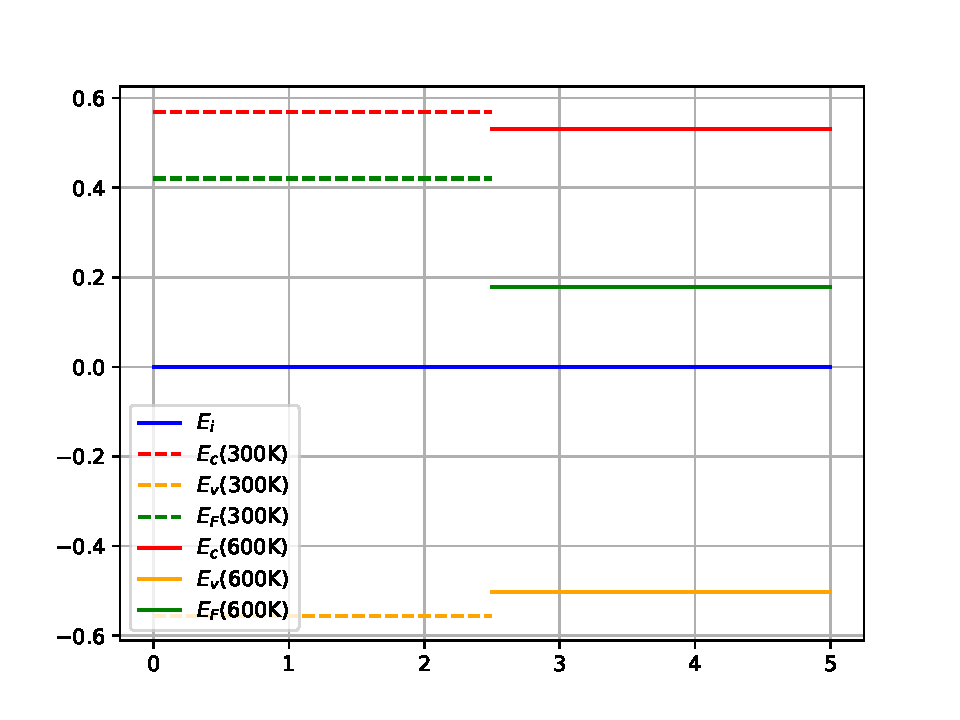
\includegraphics[width=0.9\linewidth]{Cuerpo/Ch_01/Ejercicio_01_7.pdf}
	\end{center}
